\documentclass[11pt,a4paper]{article}

\usepackage[utf8]{inputenc}
\usepackage[T1]{fontenc}
\usepackage[margin=1in]{geometry}
\usepackage{graphicx}
\usepackage{xcolor}
\usepackage{hyperref}
\usepackage{enumitem}
\usepackage{tabularx}
\usepackage{booktabs}
\usepackage{longtable}
\usepackage{listings}
\usepackage{titlesec}
\usepackage{fancyhdr}
\usepackage{caption}

\definecolor{primary}{HTML}{1F3A68}
\definecolor{accent}{HTML}{4A6FA5}
\definecolor{codebg}{HTML}{F5F7FA}

\hypersetup{
    colorlinks=true,
    linkcolor=primary,
    urlcolor=accent,
    citecolor=primary,
}

\titleformat{\section}
  {\Large\bfseries\color{primary}}{\thesection}{1em}{}
\titleformat{\subsection}
  {\large\bfseries\color{primary}}{\thesubsection}{1em}{}
\titleformat{\subsubsection}
  {\normalsize\bfseries\color{accent}}{\thesubsubsection}{1em}{}

\pagestyle{fancy}
\fancyhf{}
\rhead{\textcolor{primary}{Campus Facility Booking System}}
\lhead{\textcolor{primary}{DBMS Project Report}}
\rfoot{\thepage}

\lstset{
    basicstyle=\ttfamily\footnotesize,
    backgroundcolor=\color{codebg},
    breaklines=true,
    frame=single,
    rulecolor=\color{accent!30},
    keywordstyle=\color{primary}\bfseries,
    commentstyle=\color{gray},
    stringstyle=\color{accent},
}

\title{
    \vspace{-1cm}
    \textbf{\Huge\textcolor{primary}{Campus Facility Booking System}}\\[0.3cm]
    \Large A Final-Year DBMS Project\\[0.2cm]
    \large PostgreSQL + FastAPI + Raw SQL
}
\author{}
\date{}

\begin{document}

\maketitle
\thispagestyle{empty}

\vspace{0.5cm}
\begin{center}
\rule{0.6\textwidth}{0.5pt}
\end{center}

\tableofcontents
\thispagestyle{empty}
\newpage
\setcounter{page}{1}

% =====================================================================
\section{Introduction}

The \textbf{Campus Facility Booking System} is a final-year DBMS project that lets students, faculty, organizations, and administrators on a university campus book shared facilities such as seminar halls, labs, sports courts, guest rooms, and outdoor venues. The system is built around a wallet-based payment model, role-based access control, and strict ACID guarantees enforced at the database level.

The goal of the project is to demonstrate practical application of:
\begin{itemize}[leftmargin=*]
    \item Relational schema design with normalization up to \textbf{3NF}.
    \item ACID transactions with \textbf{atomicity}, \textbf{consistency}, \textbf{isolation}, and \textbf{durability}.
    \item Database-level integrity using \texttt{CHECK} constraints, \texttt{UNIQUE} indexes, foreign keys with \texttt{ON DELETE} policies, and PL/pgSQL triggers.
    \item Concurrency control with row-level locking (\texttt{SELECT FOR UPDATE}) and PostgreSQL \texttt{advisory locks} to enforce serializable behaviour for booking races.
    \item Indexed lookups on frequently-queried columns to keep response time low.
\end{itemize}

\subsection{Technology Stack}

\begin{table}[h]
\centering
\begin{tabularx}{0.8\textwidth}{lX}
\toprule
\textbf{Layer} & \textbf{Technology} \\
\midrule
Backend         & Python 3.10+, FastAPI, psycopg2 (raw SQL, no ORM) \\
Database        & PostgreSQL 16 \\
Frontend        & Vanilla HTML / CSS / JavaScript (single-page app) \\
Testing         & pytest, httpx, ThreadPoolExecutor for concurrency \\
\bottomrule
\end{tabularx}
\caption{Technology stack}
\end{table}

The deliberate choice of \textbf{raw SQL over an ORM} is to keep the database logic visible and to allow direct demonstration of SQL features such as triggers, constraints, advisory locks, and partial unique indexes.

\subsection{User Types and Sample Credentials}

The system supports four user roles, distinguished by the \texttt{base\_type} column in the \texttt{Users} table.

\begin{table}[h]
\centering
\begin{tabularx}{\textwidth}{llX}
\toprule
\textbf{Role} & \textbf{Count (seeded)} & \textbf{Capabilities} \\
\midrule
Student        & 30 & Login, top-up wallet, book most facilities, cancel own bookings, view own transactions. \\
Faculty        & 8  & Same as students. \\
Organization   & 10 & All of the above + can book restricted grounds (OAT, Pronite Ground). \\
Admin          & 2  & All of the above + view all transactions across users, view facility utilization reports, take facilities offline. \\
\bottomrule
\end{tabularx}
\caption{User roles and their capabilities}
\end{table}

\subsubsection{Sample Login Credentials}

The seed script (\texttt{seed.py}) populates 50 users and writes \texttt{credentials.txt} with their email + password. Passwords follow the format \textbf{4 lowercase letters + 4 digits} (enforced by a database \texttt{CHECK} constraint).

\begin{table}[h]
\centering
\begin{tabularx}{\textwidth}{llX}
\toprule
\textbf{Role} & \textbf{Email} & \textbf{Password (example)} \\
\midrule
Admin           & \texttt{admin1@iitk.ac.in}              & see \texttt{credentials.txt} \\
Admin           & \texttt{admin2@iitk.ac.in}              & see \texttt{credentials.txt} \\
Student         & \texttt{aryan.maharaj91@iitk.ac.in}     & see \texttt{credentials.txt} \\
Student         & \texttt{ayushman.chander81@iitk.ac.in}  & see \texttt{credentials.txt} \\
Organization    & \texttt{antaragni@orgs.iitk.ac.in}      & see \texttt{credentials.txt} \\
Faculty         & any \texttt{*@faculty.iitk.ac.in}       & see \texttt{credentials.txt} \\
\bottomrule
\end{tabularx}
\caption{Sample login credentials}
\end{table}

\subsection{Available Facilities}

The system models 15 distinct facilities across 7 types:

\begin{table}[h]
\centering
\begin{tabularx}{\textwidth}{llX}
\toprule
\textbf{Type} & \textbf{Count} & \textbf{Examples} \\
\midrule
\texttt{Seminar\_Hall}        & 2 & Main Seminar Hall, North Block Seminar Hall \\
\texttt{Lab}                  & 3 & CS Lab 1, CS Lab 2, Electronics Lab \\
\texttt{SAC\_Court}           & 3 & Basketball, Badminton, Tennis \\
\texttt{OAT}                  & 1 & Open Air Theatre (Org-only) \\
\texttt{Pronite\_Ground}      & 1 & Pronite Main Ground (Org-only) \\
\texttt{Hall\_Guest\_Room}    & 4 & Hall 1--4 Guest Rooms (with per-hall room numbers) \\
\texttt{Visitor\_Hostel\_Room} & 1 & Visitor Hostel (with rooms VH-101 through VH-120) \\
\bottomrule
\end{tabularx}
\caption{Facility catalogue}
\end{table}

Each facility has 8 recurring time slots (06:00 to 22:00, in 2-hour blocks) with prices ranging from Rs.0 (free, early morning) to Rs.500 (peak evening).

% =====================================================================
\newpage
\section{Database Schema}

The schema is organized into five conceptual layers. All tables are in \textbf{Third Normal Form (3NF)}: every non-key attribute depends on the entire primary key and only the primary key. There are no transitive dependencies (e.g.\ student-specific data lives in \texttt{Students}, not in \texttt{Users}; organization-type lives in \texttt{Organizations}). This avoids update anomalies and keeps each fact stored in exactly one place.

\subsection{Layer 1: Identity and Finance}

\subsubsection{\texttt{Users}}

The single source of truth for any login. Each row carries shared columns; role-specific data lives in subtype tables (\texttt{Students}, \texttt{Organizations}).

\begin{lstlisting}[language=SQL]
CREATE TABLE Users (
    user_id        SERIAL PRIMARY KEY,
    name           VARCHAR(100) NOT NULL,
    email          VARCHAR(100) UNIQUE NOT NULL,
    password       VARCHAR(100) NOT NULL DEFAULT 'xxxx0000'
                   CHECK (password ~ '^[A-Za-z]{4}[0-9]{4}$'),
    base_type      VARCHAR(20)  NOT NULL
                   CHECK (base_type IN ('Student','Faculty','Admin','Organization')),
    wallet_balance NUMERIC(10,2) NOT NULL DEFAULT 0.00
                   CHECK (wallet_balance >= 0),
    created_at     TIMESTAMP NOT NULL DEFAULT CURRENT_TIMESTAMP
);
\end{lstlisting}

\textbf{Constraints explained:}
\begin{itemize}[leftmargin=*]
    \item \texttt{email UNIQUE} — no two users can share an email.
    \item \texttt{password} regex check — enforces format \texttt{[A-Za-z]\{4\}[0-9]\{4\}}.
    \item \texttt{base\_type IN (...)} — only the four allowed roles.
    \item \texttt{wallet\_balance >= 0} — invariant: wallet never goes negative, ever.
\end{itemize}

\subsubsection{\texttt{Students} and \texttt{Organizations}}

\begin{lstlisting}[language=SQL]
CREATE TABLE Students (
    user_id     INT PRIMARY KEY REFERENCES Users(user_id) ON DELETE CASCADE,
    roll_number VARCHAR(20) UNIQUE NOT NULL
);

CREATE TABLE Organizations (
    user_id  INT PRIMARY KEY REFERENCES Users(user_id) ON DELETE CASCADE,
    org_type VARCHAR(50) NOT NULL
             CHECK (org_type IN ('Club','Festival_Committee','Society'))
);
\end{lstlisting}

\textbf{Foreign-key design:} \texttt{user\_id} is both the primary key and a foreign key to \texttt{Users}. Using \texttt{ON DELETE CASCADE} means deleting a user automatically removes their subtype row — the subtype row exists \emph{only} as a refinement of the user.

\subsubsection{\texttt{Wallet\_Transactions}}

\begin{lstlisting}[language=SQL]
CREATE TABLE Wallet_Transactions (
    transaction_id   SERIAL PRIMARY KEY,
    user_id          INT NOT NULL REFERENCES Users(user_id) ON DELETE CASCADE,
    amount           NUMERIC(10,2) NOT NULL CHECK (amount > 0),
    transaction_type VARCHAR(20) NOT NULL
                     CHECK (transaction_type IN ('Deposit','Payment','Refund')),
    description      TEXT,
    created_at       TIMESTAMP NOT NULL DEFAULT CURRENT_TIMESTAMP
);
\end{lstlisting}

This is an \textbf{immutable ledger} — once a row is inserted, it is never updated. Together with the wallet-balance invariant, this guarantees auditability: the sum of \texttt{amount * sign(transaction\_type)} over all rows for a user equals their current wallet balance.

\subsection{Layer 2: Inventory}

\subsubsection{\texttt{Facilities}, \texttt{Facility\_Rooms}, \texttt{Facility\_Slots}}

\begin{lstlisting}[language=SQL]
CREATE TABLE Facilities (
    facility_id    SERIAL PRIMARY KEY,
    name           VARCHAR(100) NOT NULL,
    type           VARCHAR(30) NOT NULL CHECK (type IN (...)),
    capacity       INTEGER NOT NULL CHECK (capacity > 0),
    is_operational BOOLEAN NOT NULL DEFAULT TRUE,
    created_at     TIMESTAMP NOT NULL DEFAULT CURRENT_TIMESTAMP
);

CREATE TABLE Facility_Rooms (
    room_id        SERIAL PRIMARY KEY,
    facility_id    INT NOT NULL REFERENCES Facilities(facility_id) ON DELETE CASCADE,
    hall_number    INTEGER,
    room_number    VARCHAR(10) NOT NULL,
    is_operational BOOLEAN NOT NULL DEFAULT TRUE,
    UNIQUE (facility_id, hall_number, room_number),
    CHECK (hall_number IS NULL OR (hall_number BETWEEN 1 AND 14))
);

CREATE TABLE Facility_Slots (
    slot_id     SERIAL PRIMARY KEY,
    facility_id INT NOT NULL REFERENCES Facilities(facility_id) ON DELETE CASCADE,
    start_time  TIME NOT NULL,
    end_time    TIME NOT NULL,
    price       NUMERIC(10,2) NOT NULL DEFAULT 0.00 CHECK (price >= 0),
    CHECK (end_time > start_time),
    UNIQUE (facility_id, start_time, end_time)
);
\end{lstlisting}

\textbf{Why three tables?} Normalization. A facility has many rooms; a facility has a recurring weekly slot template. Storing room numbers or slots inside \texttt{Facilities} would require repeating the facility's name/type/capacity for every row, violating 2NF.

\subsection{Layer 3: Booking Engine}

\subsubsection{\texttt{Bookings} and \texttt{Booking\_Slots}}

\begin{lstlisting}[language=SQL]
CREATE TABLE Bookings (
    booking_id   SERIAL PRIMARY KEY,
    user_id      INT NOT NULL REFERENCES Users(user_id) ON DELETE RESTRICT,
    booking_date DATE NOT NULL,
    total_cost   NUMERIC(10,2) NOT NULL CHECK (total_cost >= 0),
    status       VARCHAR(20) NOT NULL
                 CHECK (status IN ('Pending','Confirmed','Cancelled')),
    created_at   TIMESTAMP NOT NULL DEFAULT CURRENT_TIMESTAMP
);

CREATE TABLE Booking_Slots (
    booking_slot_id SERIAL PRIMARY KEY,
    booking_id      INT NOT NULL REFERENCES Bookings(booking_id) ON DELETE CASCADE,
    slot_id         INT NOT NULL REFERENCES Facility_Slots(slot_id) ON DELETE RESTRICT,
    room_id         INT REFERENCES Facility_Rooms(room_id) ON DELETE RESTRICT,
    price_charged   NUMERIC(10,2) NOT NULL CHECK (price_charged >= 0)
);

CREATE UNIQUE INDEX uq_booking_slots_with_room
    ON Booking_Slots (booking_id, slot_id, room_id) WHERE room_id IS NOT NULL;
CREATE UNIQUE INDEX uq_booking_slots_no_room
    ON Booking_Slots (booking_id, slot_id) WHERE room_id IS NULL;
\end{lstlisting}

\textbf{Key design choices:}
\begin{itemize}[leftmargin=*]
    \item \texttt{ON DELETE RESTRICT} on \texttt{Bookings.user\_id} — prevents deleting a user who has booking history. Bookings are an audit record.
    \item \texttt{ON DELETE CASCADE} on \texttt{Booking\_Slots.booking\_id} — line items only exist as part of a booking; if the booking is hard-deleted (rare; we usually \texttt{Cancel} instead), the line items go with it.
    \item Two \textbf{partial unique indexes} on \texttt{Booking\_Slots} — prevent the same slot appearing twice in one cart, with NULL-aware semantics. Standard \texttt{UNIQUE} treats two NULL \texttt{room\_id}s as distinct, which would let duplicates slip through; partial indexes split the world into "with room" and "without room" cases.
\end{itemize}

\subsection{Layer 4: Database-Level Enforcement (Triggers)}

\subsubsection{Trigger 1: \texttt{validate\_ground\_booking}}

Only \texttt{Organization} users can book OAT or Pronite Ground. Enforced as a \texttt{BEFORE INSERT/UPDATE} trigger on \texttt{Booking\_Slots}.

\begin{lstlisting}[language=SQL]
CREATE OR REPLACE FUNCTION validate_ground_booking()
RETURNS TRIGGER AS $$
DECLARE u_base_type VARCHAR; fac_type VARCHAR;
BEGIN
    SELECT f.type INTO fac_type
      FROM Facilities f JOIN Facility_Slots fs ON f.facility_id = fs.facility_id
     WHERE fs.slot_id = NEW.slot_id;
    SELECT u.base_type INTO u_base_type
      FROM Users u JOIN Bookings b ON u.user_id = b.user_id
     WHERE b.booking_id = NEW.booking_id;
    IF fac_type IN ('OAT','Pronite_Ground') AND u_base_type <> 'Organization' THEN
        RAISE EXCEPTION 'Access Denied: Only official Organizations can book major grounds.';
    END IF;
    RETURN NEW;
END;
$$ LANGUAGE plpgsql;
\end{lstlisting}

\subsubsection{Trigger 2: \texttt{prevent\_double\_booking}}

The most important integrity rule: no two bookings can hold the same \texttt{slot\_id} on the same \texttt{booking\_date} (cancelled bookings are ignored). Combined with application-side advisory locks, this gives serializable booking behaviour.

\begin{lstlisting}[language=SQL]
CREATE OR REPLACE FUNCTION prevent_double_booking()
RETURNS TRIGGER AS $$
DECLARE new_date DATE; conflict INT;
BEGIN
    SELECT booking_date INTO new_date FROM Bookings WHERE booking_id = NEW.booking_id;
    SELECT COUNT(*) INTO conflict
      FROM Booking_Slots bs JOIN Bookings b ON b.booking_id = bs.booking_id
     WHERE bs.slot_id = NEW.slot_id AND b.booking_date = new_date
       AND b.status IN ('Pending','Confirmed') AND bs.booking_id <> NEW.booking_id
       AND COALESCE(bs.room_id, -1) = COALESCE(NEW.room_id, -1);
    IF conflict > 0 THEN
        RAISE EXCEPTION 'Slot % on % is already booked.', NEW.slot_id, new_date;
    END IF;
    RETURN NEW;
END;
$$ LANGUAGE plpgsql;
\end{lstlisting}

\subsection{Layer 5: Performance Indexing}

Indexes accelerate the most frequent queries the API issues:

\begin{table}[h]
\centering
\begin{tabularx}{\textwidth}{llX}
\toprule
\textbf{Index} & \textbf{Table} & \textbf{Why} \\
\midrule
\texttt{idx\_facility\_slots\_facility} & \texttt{Facility\_Slots(facility\_id)} & Availability lookup is always filtered by facility. \\
\texttt{idx\_bookings\_date\_status} & \texttt{Bookings(booking\_date, status)} & Admin utilization report and availability checks scan by date+status. \\
\texttt{idx\_booking\_slots\_slot} & \texttt{Booking\_Slots(slot\_id)} & The double-booking trigger queries Booking\_Slots by slot\_id — without this, every insert would scan the table. \\
\texttt{idx\_wallet\_tx\_user\_time} & \texttt{Wallet\_Transactions(user\_id, created\_at DESC)} & "My Transactions" page sorts a user's ledger newest-first. \\
\texttt{idx\_facility\_rooms\_facility} & \texttt{Facility\_Rooms(facility\_id)} & Room dropdown listing for hall guest rooms / visitor hostel. \\
\bottomrule
\end{tabularx}
\caption{Indexes for performance}
\end{table}

\subsection{Concurrency Control: Serializability}

PostgreSQL's default \texttt{READ COMMITTED} isolation level is too weak for the booking workflow — two concurrent transactions can both see "no conflict" because neither has committed yet. Three layers ensure correct serializable behaviour:

\begin{enumerate}[leftmargin=*]
    \item \textbf{Advisory locks (application layer)}: \texttt{create\_booking} calls \texttt{pg\_advisory\_xact\_lock(slot\_id, date\_int)} before any inserts. Concurrent requests for the same slot+date queue at this lock; the second only proceeds after the first commits or rolls back.
    \item \textbf{Row-level locks (financial layer)}: \texttt{SELECT ... FOR UPDATE} on the user's row before reading the wallet balance. This serializes wallet-spending decisions for the same user.
    \item \textbf{Trigger-based check (defense in depth)}: even if locks failed, the \texttt{prevent\_double\_booking} trigger sees committed conflicts and raises an exception, rolling back the transaction.
\end{enumerate}

% =====================================================================
\newpage
\section{User Interface}

This section presents screenshots of the major screens. The application is a single-page app served from \texttt{static/index.html}, communicating with the FastAPI backend over JSON.

\subsection{Login Screen}

\begin{figure}[h]
\centering
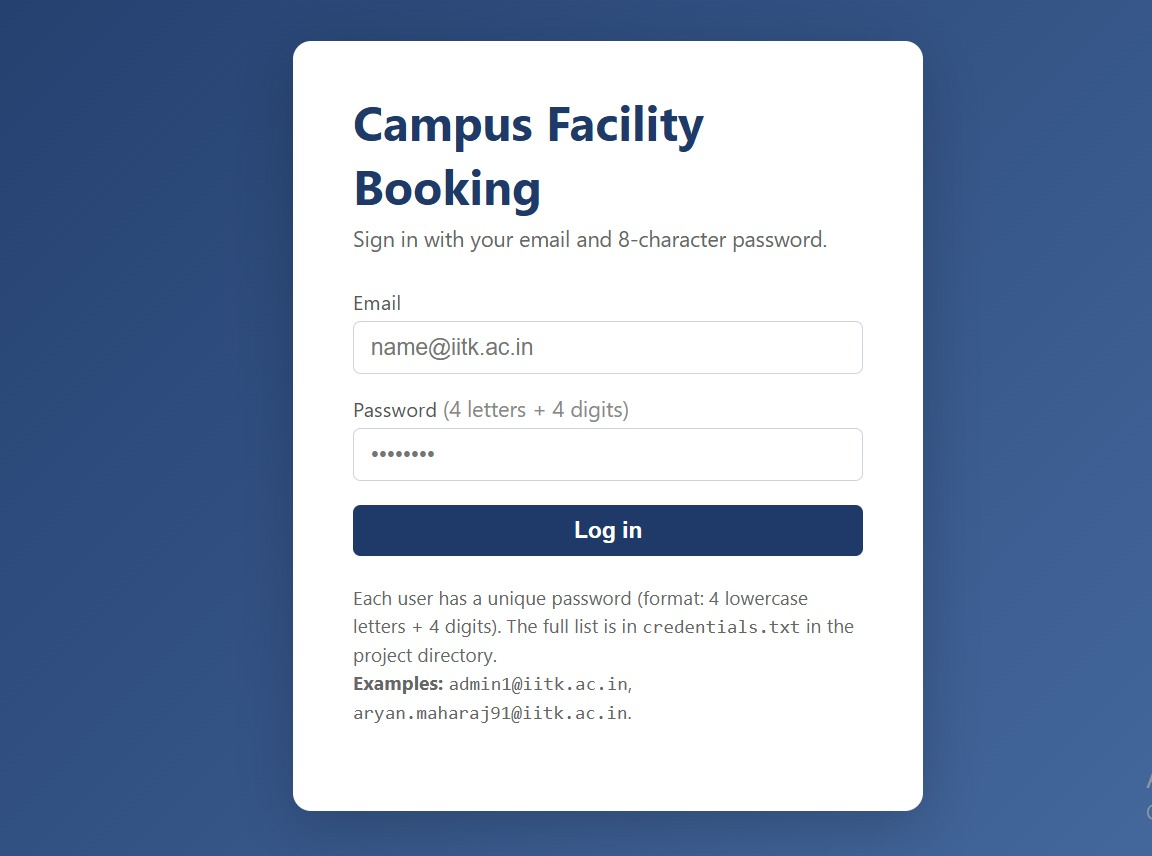
\includegraphics[width=0.7\textwidth]{../images/login-screen.jpg}
\caption{Login screen. Users authenticate with their campus email and an 8-character password (4 letters + 4 digits, enforced by a \texttt{CHECK} constraint).}
\end{figure}

\subsection{Student Profile and Wallet}

\begin{figure}[h]
\centering
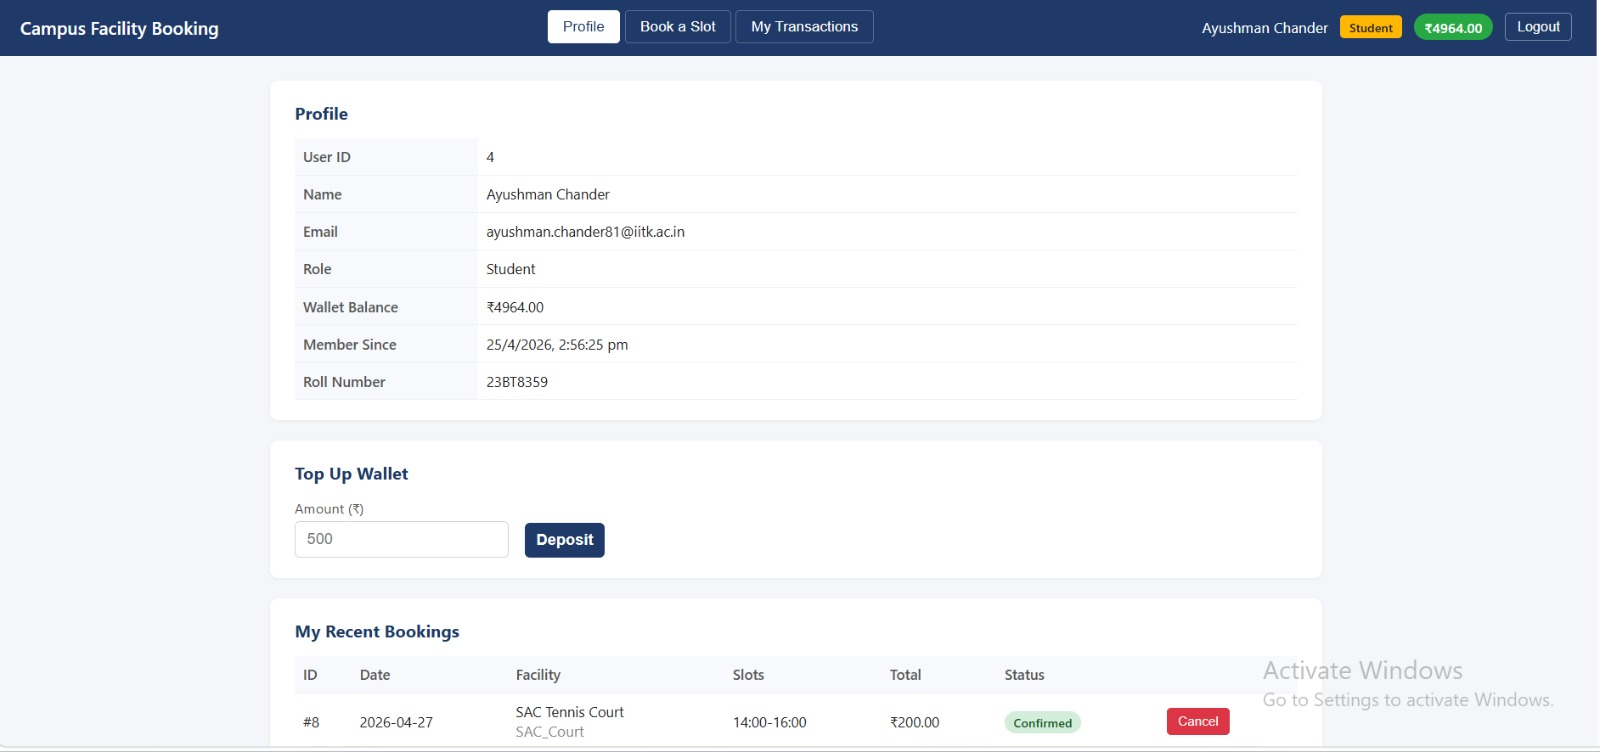
\includegraphics[width=\textwidth]{../images/profile-student.jpg}
\caption{Student profile view showing user details, wallet balance, top-up form, and recent bookings. The wallet badge in the header is refreshed on every navigation to keep the displayed balance in sync with the database.}
\end{figure}

\subsection{Booking a Facility}

\begin{figure}[h]
\centering
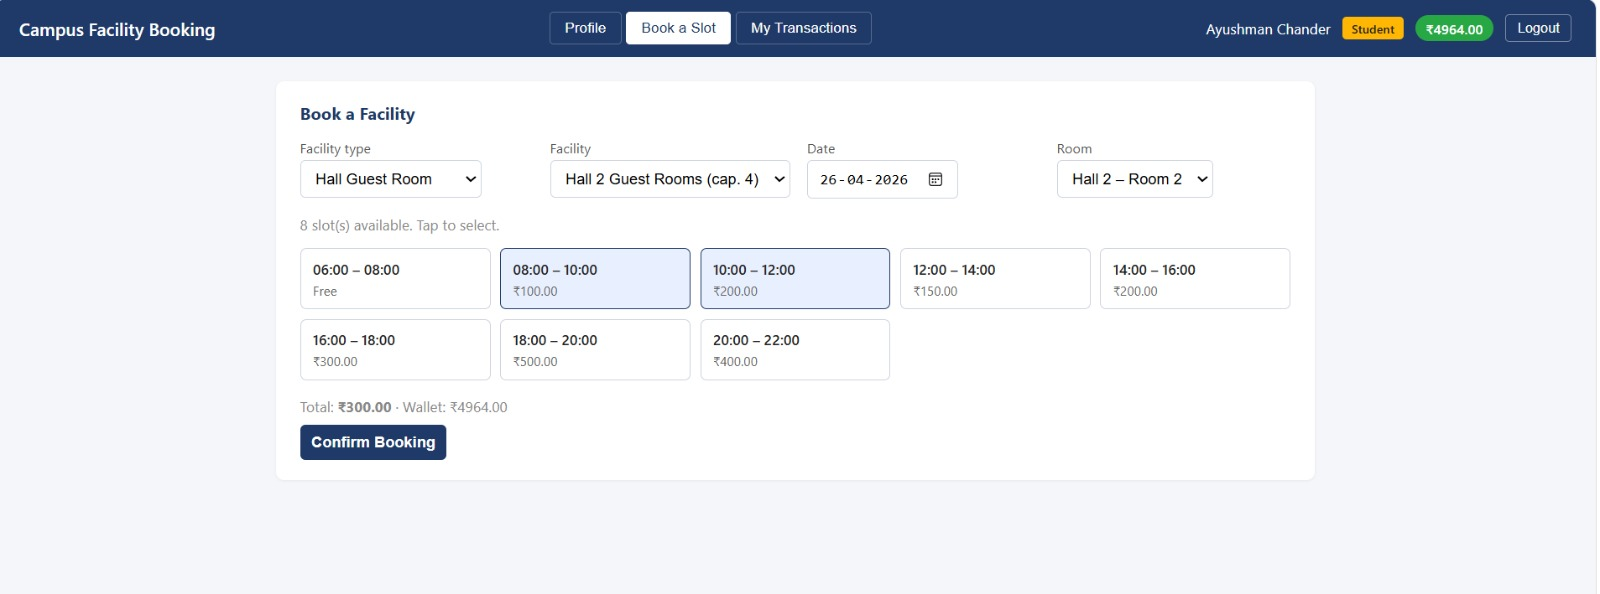
\includegraphics[width=\textwidth]{../images/book-slot.jpg}
\caption{The booking flow. The user picks a facility type, a specific facility, a date, and (for hall guest rooms or the visitor hostel) a room. Available slots are computed server-side by excluding any slot already in a Pending or Confirmed booking on that date. Selected slots are highlighted in blue; the running total updates live.}
\end{figure}

\subsection{Wallet Transactions}

\begin{figure}[h]
\centering
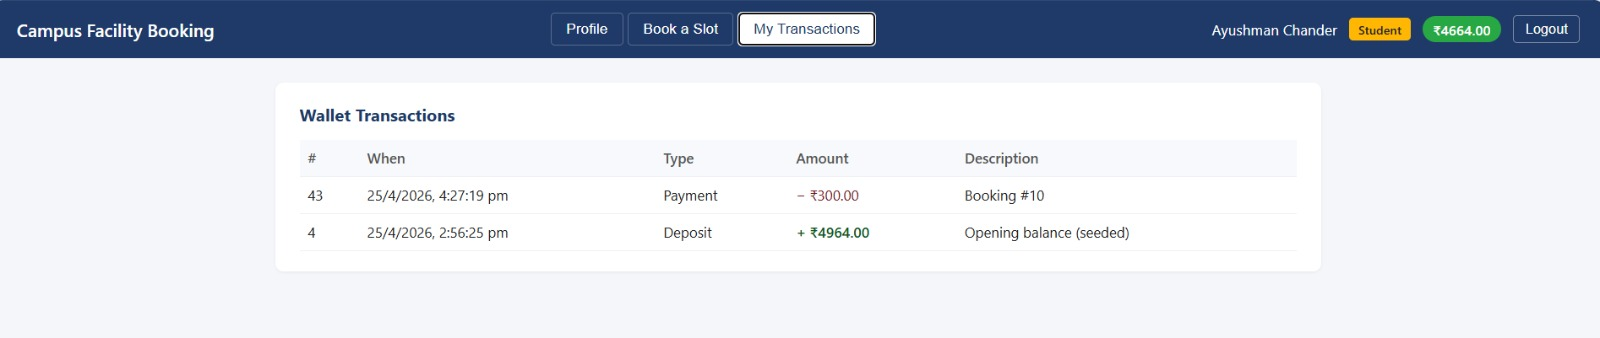
\includegraphics[width=\textwidth]{../images/my-transactions.jpg}
\caption{The user's wallet transaction ledger — every Deposit, Payment, and Refund. Sorted newest-first using the \texttt{idx\_wallet\_tx\_user\_time} index.}
\end{figure}

\subsection{Admin: All Transactions}

\begin{figure}[h]
\centering
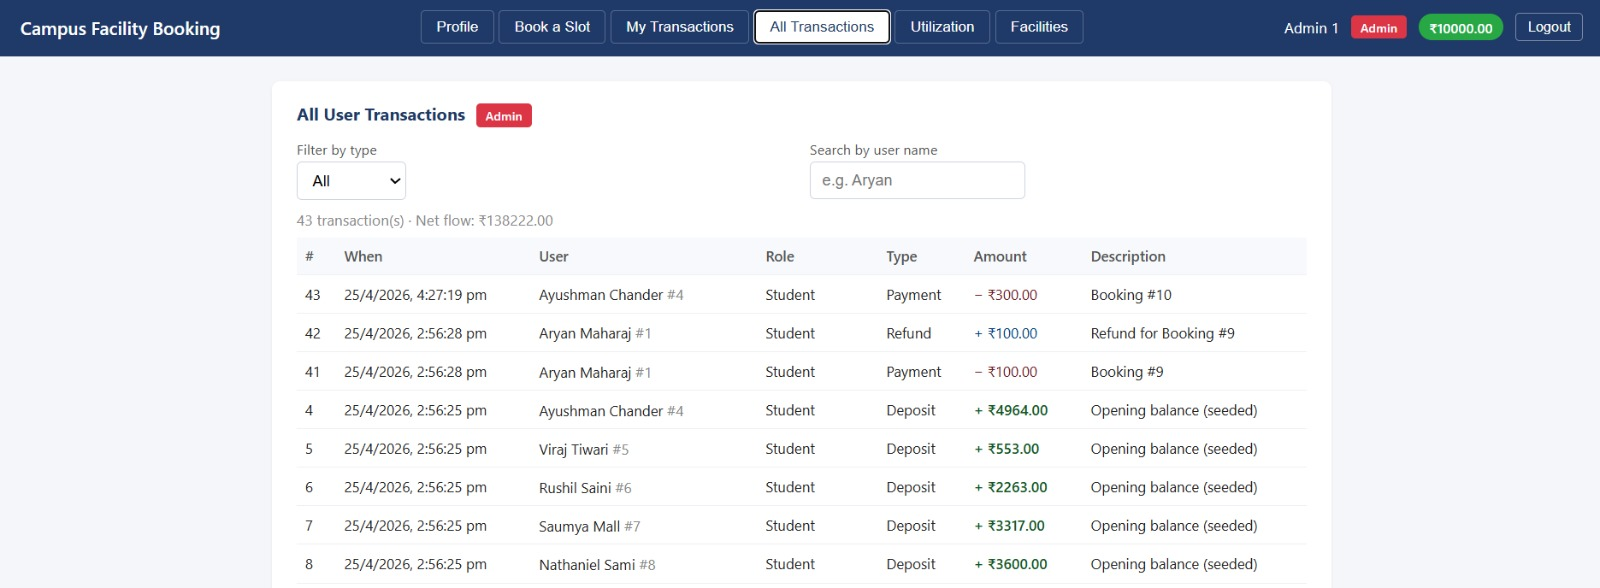
\includegraphics[width=\textwidth]{../images/admin-all-transactions.jpg}
\caption{Admin-only "All Transactions" view. Lists every wallet transaction across every user, with filters by transaction type and user name. Net flow at the top of the table aggregates Deposits + Refunds minus Payments.}
\end{figure}

\subsection{Admin: Facility Utilization Report}

\begin{figure}[h]
\centering
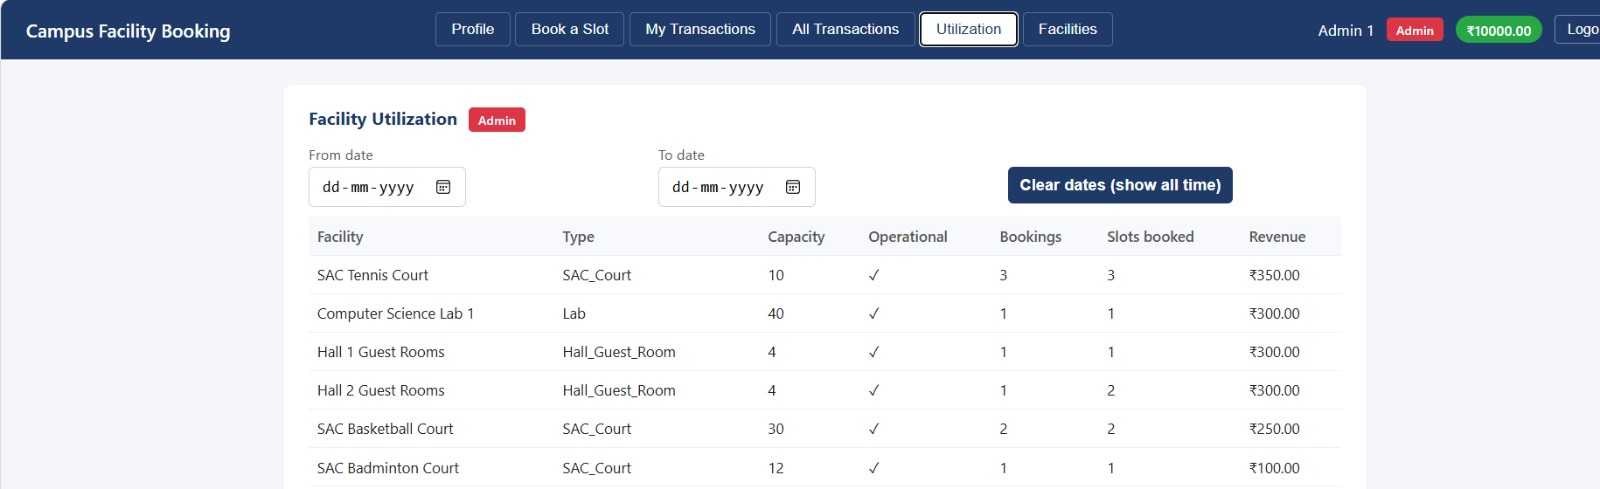
\includegraphics[width=\textwidth]{../images/admin-utilization.jpg}
\caption{Admin "Utilization" report. Shows bookings, slots booked, and revenue per facility — backed by a CTE that joins \texttt{Bookings}, \texttt{Booking\_Slots}, \texttt{Facility\_Slots}, and \texttt{Facilities} with optional date-range filters. Sorted by revenue descending.}
\end{figure}

\subsection{Admin: Facility Maintenance}

\begin{figure}[h]
\centering
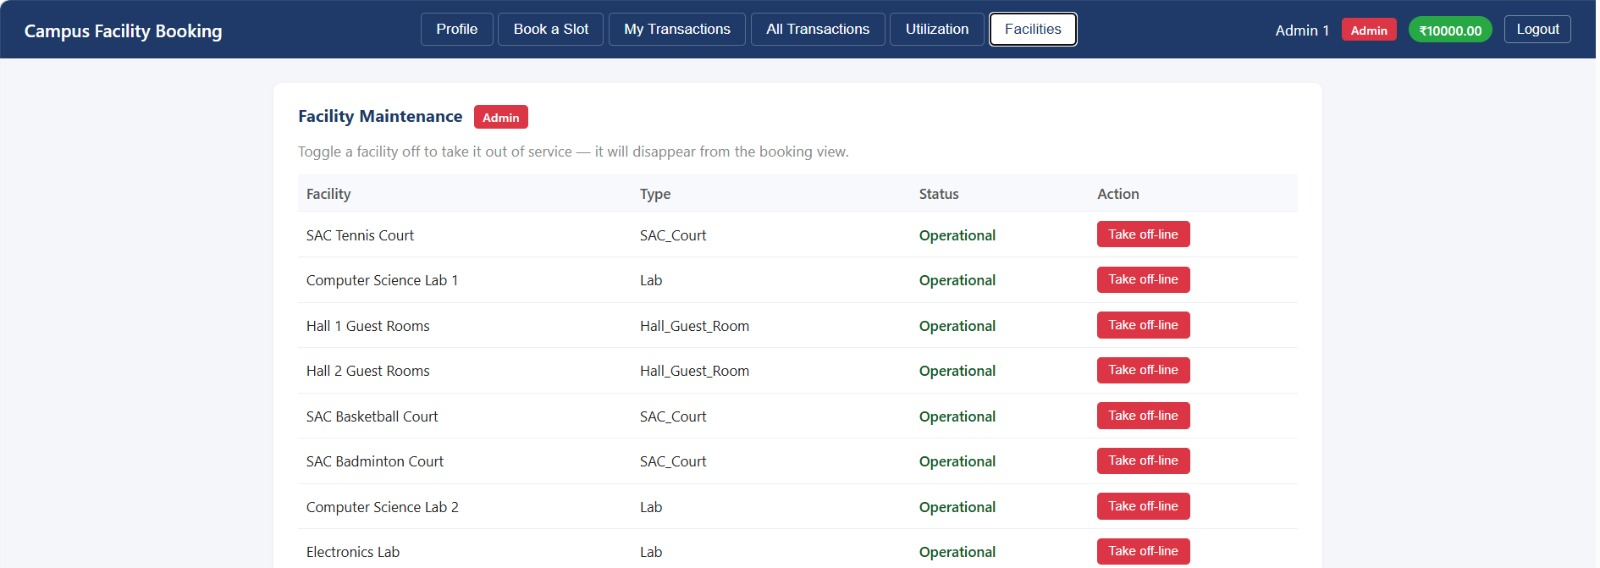
\includegraphics[width=\textwidth]{../images/admin-facilities.jpg}
\caption{Admin "Facilities" maintenance view. Toggling a facility off-line sets \texttt{is\_operational = FALSE}, which immediately removes it from the booking dropdown for non-admin users (the \texttt{/api/facilities} endpoint filters on this column).}
\end{figure}

% =====================================================================
\newpage
\section{Testing and Verification}

The project includes both a \textbf{manual UI testing plan} (\texttt{TESTING.md}) and an \textbf{automated pytest suite} of 17 tests covering all four ACID properties.

\begin{figure}[h]
\centering
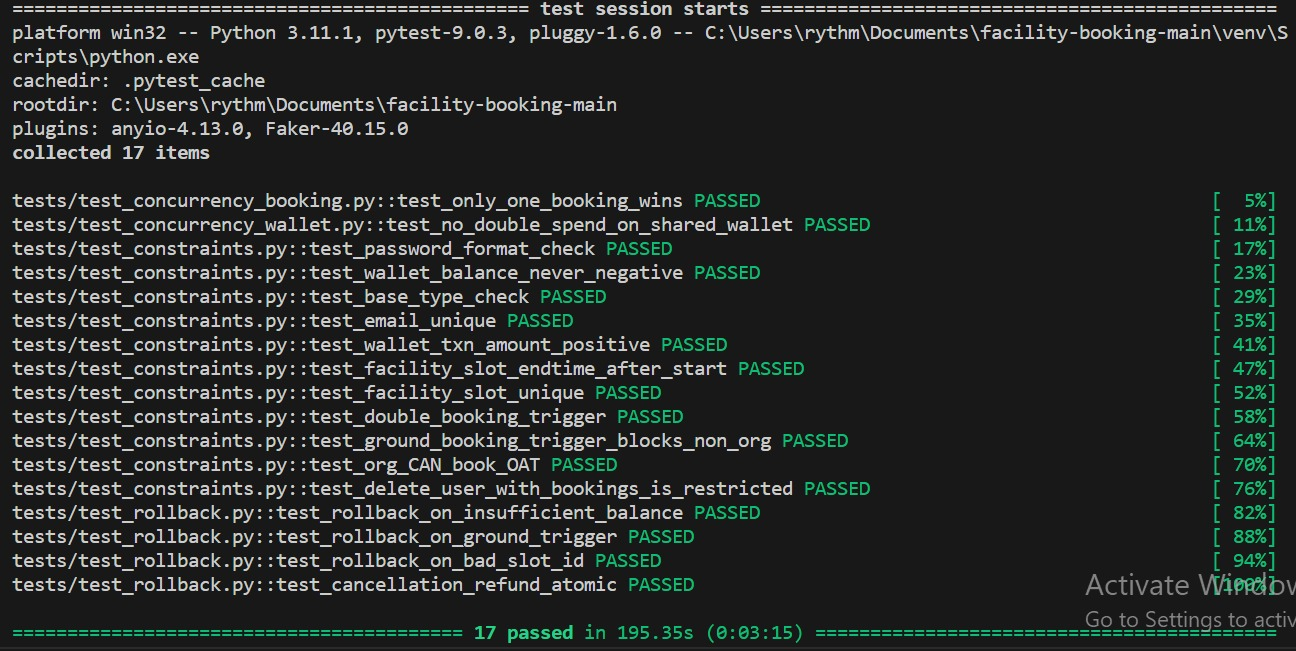
\includegraphics[width=\textwidth]{../images/pytest-results.jpg}
\caption{All 17 automated tests passing in 195 seconds. Four test files cover concurrency, constraints, rollback, and the wallet double-spend scenario.}
\end{figure}

\subsection{ACID Coverage Map}

\begin{table}[h]
\centering
\begin{tabularx}{\textwidth}{lll}
\toprule
\textbf{ACID Property} & \textbf{Test File} & \textbf{Number of Tests} \\
\midrule
Atomicity     & \texttt{test\_rollback.py}            & 4 \\
Consistency   & \texttt{test\_constraints.py}         & 11 \\
Isolation     & \texttt{test\_concurrency\_booking.py}, \texttt{test\_concurrency\_wallet.py} & 2 \\
Durability    & All 17 tests (every assertion reads back from DB) & implicit \\
\bottomrule
\end{tabularx}
\caption{Mapping of automated tests to ACID properties}
\end{table}

\subsection{Concurrency Tests (Isolation)}

\subsubsection{\texttt{test\_only\_one\_booking\_wins}}

\textbf{Purpose:} Prove that exactly 1 of N concurrent bookings of the same slot succeeds.

\textbf{Setup:} 30 student bots are loaded from \texttt{credentials.txt}, each with $\geq$ Rs.1000 wallet balance. The first available slot on a target facility/date is identified.

\textbf{Action:} Using \texttt{ThreadPoolExecutor(max\_workers=30)}, all 30 bots fire \texttt{POST /api/bookings} for that slot at the same instant.

\textbf{Expected:} 1 winner (HTTP 201). 29 losses (HTTP 400 with "Slot X on date is already booked"). DB query confirms exactly 1 live \texttt{Booking\_Slots} row.

\textbf{What it proves:} Without protection, two transactions in \texttt{READ COMMITTED} could both pass the \texttt{prevent\_double\_booking} trigger check (since neither sees the other's uncommitted insert) and both succeed. The combination of \texttt{pg\_advisory\_xact\_lock} (serializing access) and the trigger (rejecting confirmed conflicts) guarantees exactly one winner.

\subsubsection{\texttt{test\_no\_double\_spend\_on\_shared\_wallet}}

\textbf{Purpose:} Prove that \texttt{SELECT FOR UPDATE} prevents over-spending under concurrency.

\textbf{Setup:} One student's wallet is reset to exactly Rs.500. Twenty distinct Rs.200 slots (across multiple non-restricted facilities) are picked. Twenty separate \texttt{Bot} instances all log in as the same student.

\textbf{Action:} 20 concurrent \texttt{POST /api/bookings} requests are fired in parallel.

\textbf{Expected:} Exactly $\lfloor 500/200 \rfloor = 2$ bookings succeed; 18 fail with "insufficient balance"; final wallet balance is exactly Rs.100; \texttt{Wallet\_Transactions} payment count equals winners.

\textbf{What it proves:} The \texttt{SELECT user\_id, wallet\_balance FROM Users WHERE user\_id = \%s FOR UPDATE} statement acquires a row-level exclusive lock on the user row. Concurrent transactions block at this lock and re-read the now-debited wallet, ensuring \texttt{wallet\_balance} never goes negative.

\subsection{Rollback / Atomicity Tests}

\subsubsection{\texttt{test\_rollback\_on\_insufficient\_balance}}

A student with Rs.10 attempts to book a Rs.500 slot. The endpoint snapshots \texttt{(wallet, count(bookings), count(transactions))} before and after. Assertion: pre-state and post-state are byte-identical. The \texttt{conn.rollback()} on the failure path undoes the booking-header insert, so no orphan rows survive.

\subsubsection{\texttt{test\_rollback\_on\_ground\_trigger}}

A student with Rs.10000 (so balance is not the failure cause) tries to book OAT. The \texttt{validate\_ground\_booking} trigger raises mid-transaction; everything inserted before the trigger fires (the \texttt{Bookings} header) rolls back.

\subsubsection{\texttt{test\_rollback\_on\_bad\_slot\_id}}

Sending \texttt{slot\_ids: [999\_999]} causes a 400 "invalid slot ID". Verifies validation errors that fire before any insert leave the DB clean.

\subsubsection{\texttt{test\_cancellation\_refund\_atomic}}

Books a paid slot, then immediately cancels. Verifies: net wallet change = 0, bookings count +1 (cancelled but kept for history), transactions count +2 (one Payment + one Refund). The cancel endpoint touches three tables in one atomic commit.

\subsection{Constraint Tests (Consistency)}

These hit PostgreSQL directly (bypassing the API) to verify every \texttt{CHECK}, \texttt{UNIQUE}, foreign-key, and trigger fires when violated.

\begin{longtable}{lp{3.5cm}p{8cm}}
\toprule
\textbf{\#} & \textbf{Test} & \textbf{What it verifies} \\
\midrule
\endhead
9.1  & \texttt{password\_format\_check}              & Password regex \texttt{[A-Za-z]\{4\}[0-9]\{4\}}. \\
9.2  & \texttt{wallet\_balance\_never\_negative}     & \texttt{wallet\_balance >= 0}. \\
9.3  & \texttt{base\_type\_check}                    & \texttt{base\_type IN ('Student','Faculty','Admin','Organization')}. \\
9.4  & \texttt{email\_unique}                        & \texttt{Users.email UNIQUE}. \\
9.5  & \texttt{wallet\_txn\_amount\_positive}        & \texttt{Wallet\_Transactions.amount > 0}. \\
9.6  & \texttt{facility\_slot\_endtime\_after\_start} & \texttt{end\_time > start\_time}. \\
9.7  & \texttt{facility\_slot\_unique}               & \texttt{UNIQUE(facility\_id, start\_time, end\_time)}. \\
9.8  & \texttt{double\_booking\_trigger}             & \texttt{prevent\_double\_booking} fires on duplicate slot+date. \\
9.9  & \texttt{ground\_booking\_trigger\_blocks\_non\_org} & Trigger blocks a Student from booking OAT. \\
9.10 & \texttt{org\_CAN\_book\_OAT}                  & Counter-test: Organization succeeds where Student failed. \\
9.11 & \texttt{delete\_user\_with\_bookings\_is\_restricted} & \texttt{ON DELETE RESTRICT} on \texttt{Bookings.user\_id}. \\
\bottomrule
\caption{Every constraint test in test\_constraints.py}
\end{longtable}

\subsection{Test Infrastructure}

\textbf{Bot harness} (\texttt{tests/bots.py}): wraps \texttt{httpx.Client} for one logged-in user, exposing \texttt{login / profile / deposit / availability / book / cancel}. \texttt{load\_bots(n, role)} returns N pre-authenticated bots.

\textbf{Fixtures} (\texttt{tests/conftest.py}):
\begin{itemize}[leftmargin=*]
    \item \texttt{api\_url} — confirms the backend is reachable via \texttt{/api/health}; skips tests if not.
    \item \texttt{fresh\_db} — truncates only the transactional tables (\texttt{Booking\_Slots}, \texttt{Bookings}, \texttt{Wallet\_Transactions}) and resets every wallet to Rs.1000. Users and facilities are preserved across runs.
    \item \texttt{db\_conn} — a direct \texttt{psycopg2} connection in a transaction that's always rolled back at teardown. Used by constraint tests.
\end{itemize}

% =====================================================================
\newpage
\section{Conclusion}

The Campus Facility Booking System demonstrates a database-first design philosophy: as much of the business logic as possible lives in the database (constraints, triggers, indexes), with the application layer responsible only for serializing access and exposing the API.

\textbf{Key takeaways:}
\begin{itemize}[leftmargin=*]
    \item \textbf{Schema in 3NF} — no redundant attributes, every fact in exactly one place.
    \item \textbf{ACID guarantees} are not optional — every test in the suite exercises one or more of A, C, I, D.
    \item \textbf{Concurrency cannot rely on triggers alone} — \texttt{READ COMMITTED} permits the trigger check to pass for both racers. Advisory locks plus row-level \texttt{FOR UPDATE} locks fill that gap and produce serializable behaviour.
    \item \textbf{Partial unique indexes with NULL-aware predicates} elegantly solve the "same slot in multiple lines of one cart" duplication problem when \texttt{room\_id} is optional.
    \item \textbf{Audit invariants} are upheld at the database level, not by hopeful application code: \texttt{wallet\_balance >= 0}, \texttt{amount > 0}, \texttt{ON DELETE RESTRICT} on bookings.
\end{itemize}

The system has been validated through:
\begin{itemize}[leftmargin=*]
    \item 17 automated pytest tests covering concurrency, rollback, and constraint scenarios.
    \item Manual UI walkthroughs documented in \texttt{TESTING.md}.
    \item End-to-end flows shown in the screenshots above.
\end{itemize}

The codebase is intentionally minimal (\textasciitilde 600 lines of Python + \textasciitilde 250 lines of SQL + a single HTML file) to keep the database layer the centerpiece of the design.

\vspace{1cm}
\hrule
\vspace{0.3cm}
\centering
\textcolor{primary}{\textit{Source code: \href{https://github.com/be-water22/facility-booking}{github.com/be-water22/facility-booking}}}

\end{document}
